\subsection{Dokumentation af kode}
Alle metoder, klasser og konstanter er blevet beskrevet i koden løbende. Disse beskrivelse er vha. programmet Doxygen blevet omdannet til html såvel som Latex filer der på struktureret vis opstiller disse med hyperlink til hurtigt og nemt navigere mellem sektioner. Hvis yderligere kodedokumentation ønskes henvises der til disse Doxygen filer. Der kan forefindes doxygen-filer for Devkit8000\footcite{doxy-devkit}, PSoC-Master\footcite{doxy-master}, PSoC-XY\footcite{doxy-xy}, PSoC-Z\footcite{doxy-z} og PSoC-Sensor\footcite{doxy-sensor}.

% 6.1.2 Applikationsmodeller
\subsection{Applikationsmodeller}

Selve designet af softwaren bygger på de følgende applikationsmodeller. Her laves der sekvens- og klassediagrammer over hver del af systemet samt klassebeskrivelser, hvor funktionen for de enkelte metoder beskrives.

% 6.1.2.1 DevKit8000
\subsubsection{DevKit8000}

Applikationsmodel for UC1: Kalibrer system.

\begin{figure}[H] \centering
    \fbox{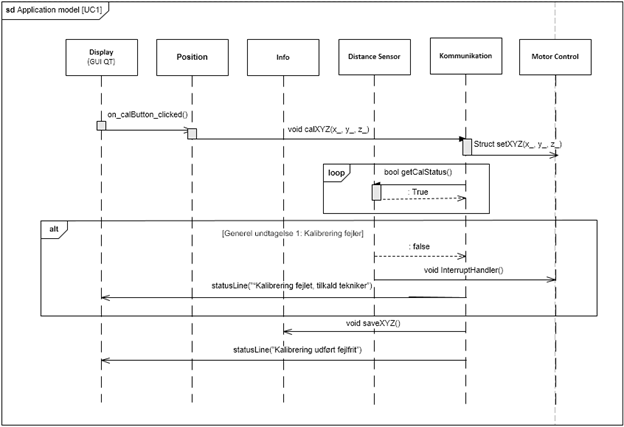
\includegraphics[width=0.95\textwidth]{0_Filer/Figuer/uc1App.png}}
    \caption{Applikationsmodel med udgangspunkt i UC1}
    \label{fig:uc1App}
\end{figure}

\begin{figure}[H] \centering
    \fbox{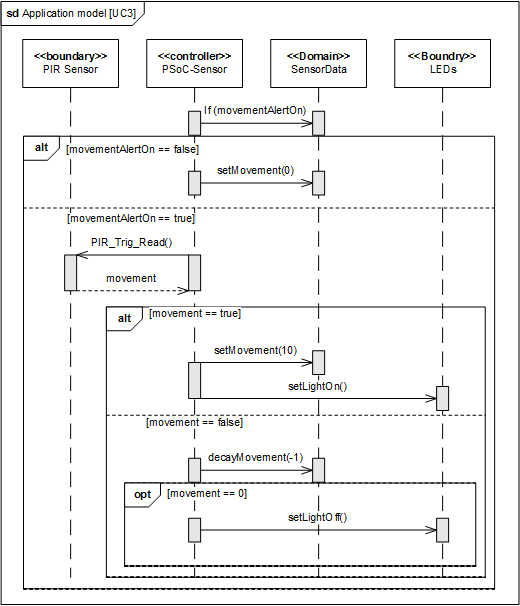
\includegraphics[width=0.95\textwidth]{0_Filer/Figuer/sdApplikationsmodelUC3-v3.png}}
    \caption{Applikationsmodel med udgangspunkt i UC3}
    \label{fig:uc3App}
\end{figure}


% 6.1.2.2 PSoC Master
\subsubsection{PSoC Master}

Applikationsmodeller for PSoC Master.

\begin{figure}[H] \centering
    \fbox{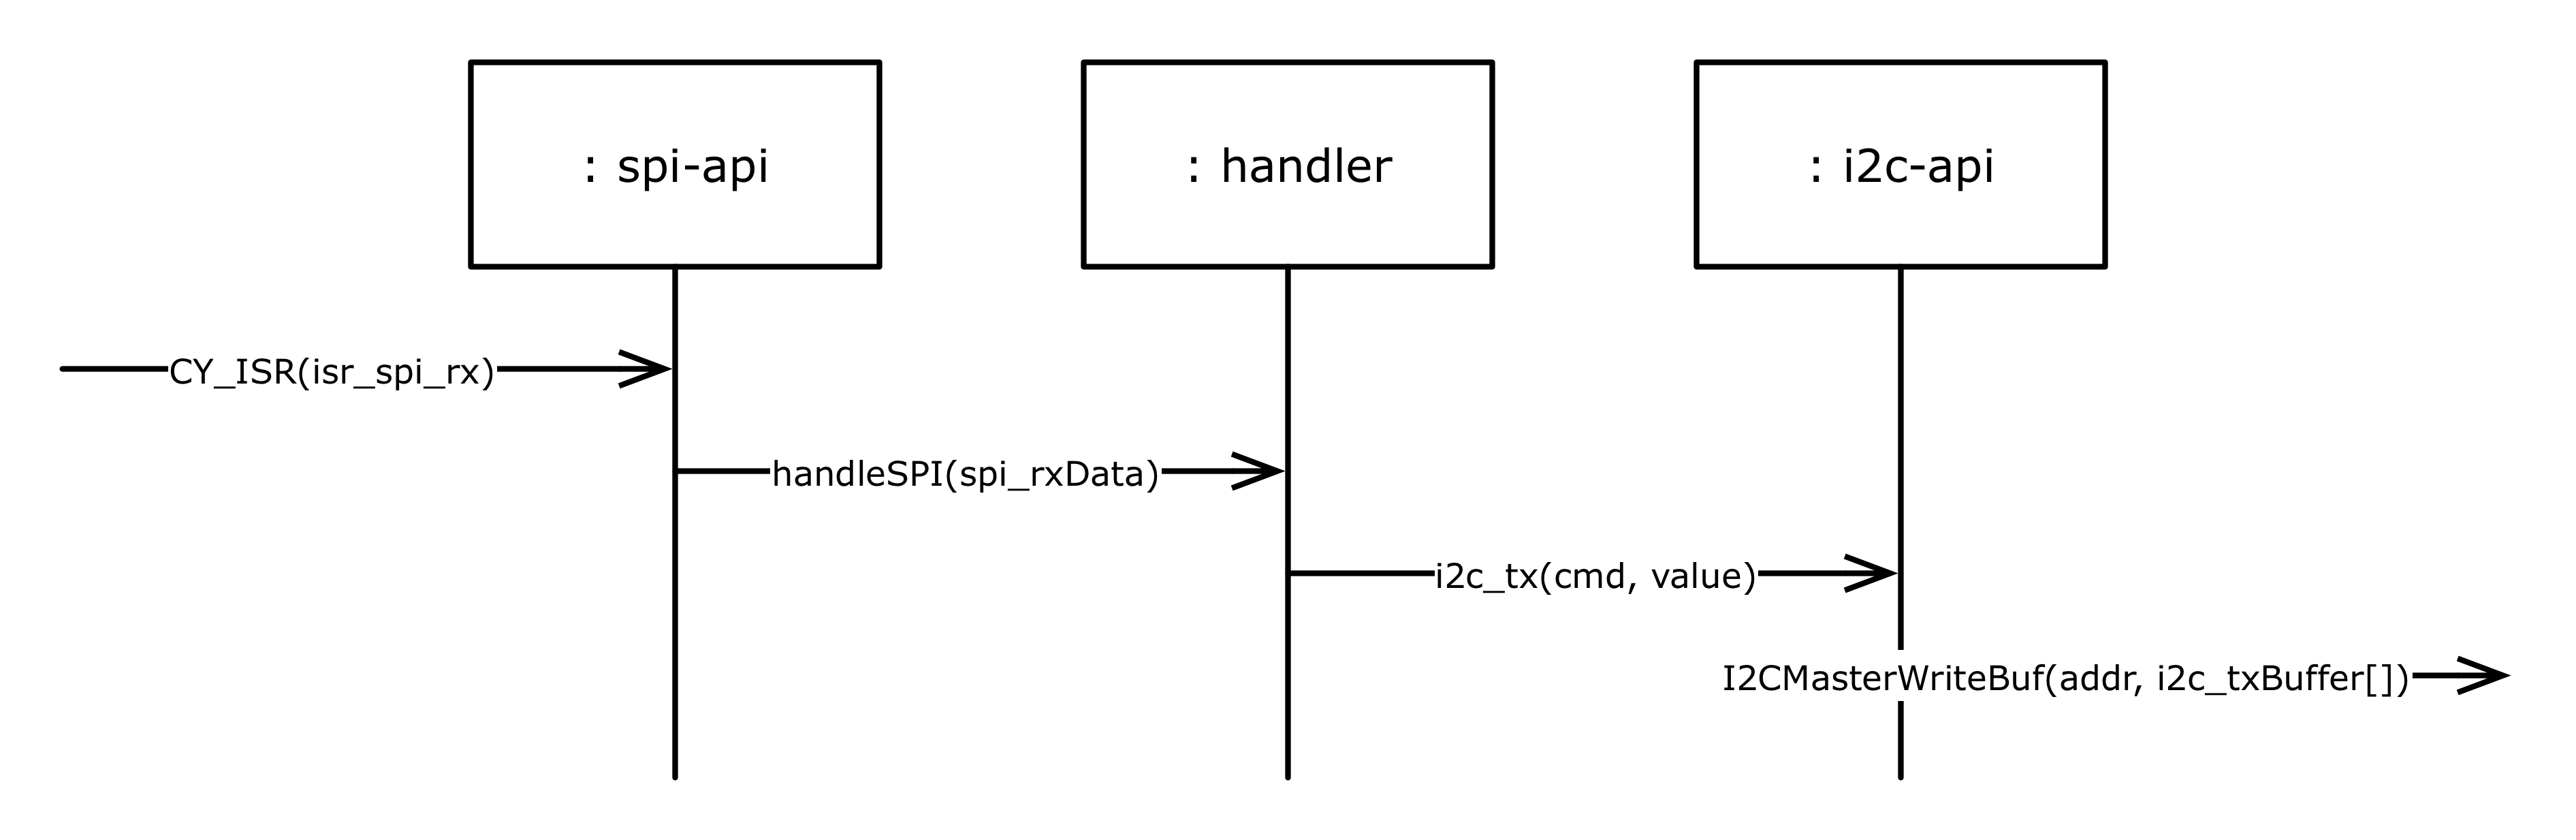
\includegraphics[width=0.95\textwidth]{0_Filer/Figuer/SPItoI2C.png}}
    \caption{Sekvensdiagram for "set" kommando via PSoC Master}
    \label{fig:sekvensdiagram_psoc_master_set}
\end{figure}

\begin{figure}[H] \centering
    \fbox{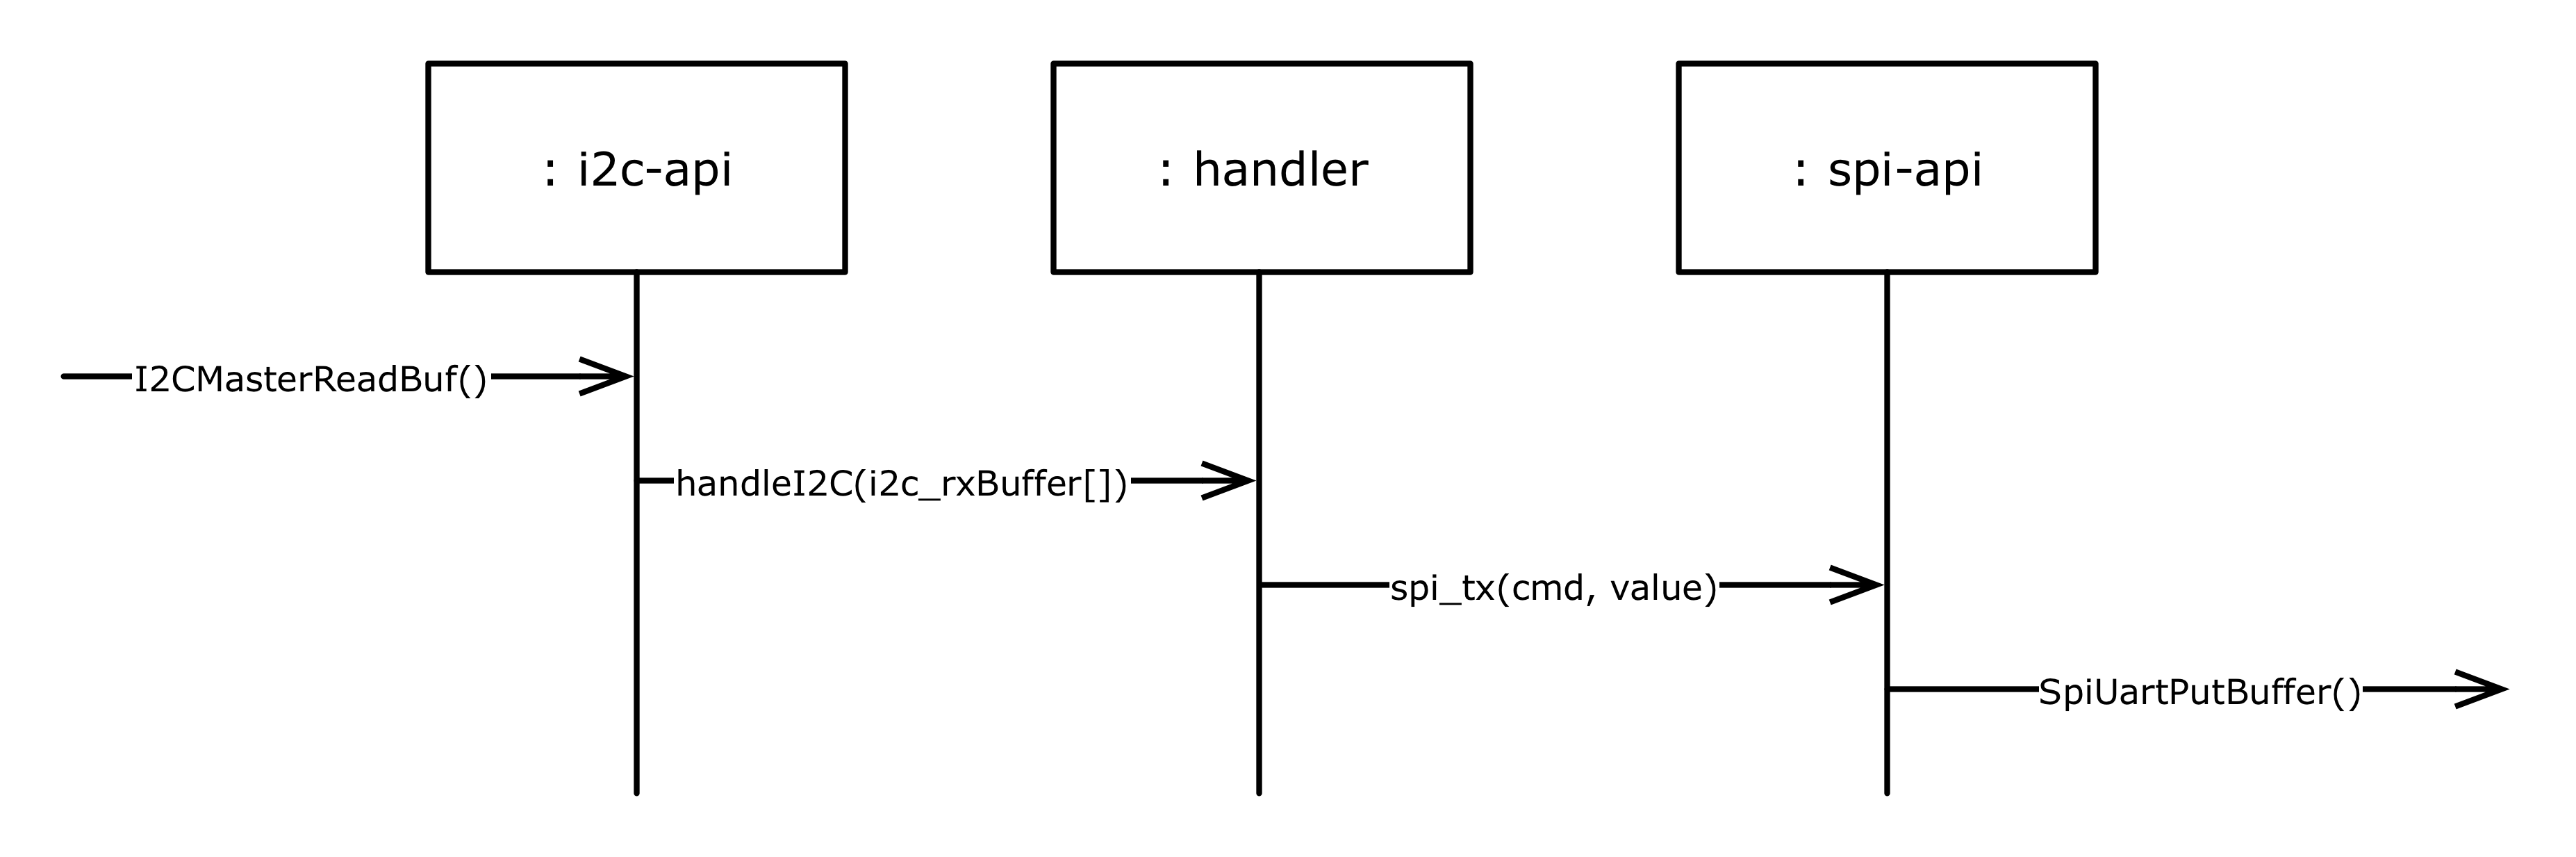
\includegraphics[width=0.95\textwidth]{0_Filer/Figuer/I2CtoSPI.png}}
    \caption{Sekvensdiagram for "get" kommando via PSoC Master}
    \label{fig:sekvensdiagram_psoc_master_get}
\end{figure}

% 6.1.2.3 Klassebeskrivelser
\subsubsection{Klassebeskrivelser PSoC Master}

Her følger klassebeskrivelser for de udledte klasser fra applikationsmodellerne.
% 6.1.2.3 Klassebeskrivelser PSoC Master

% spi-api
\begin{table}[H]
    \centering
    \begin{tabular}{|l|}
    \hline
    \multicolumn{1}{|c|}{<<boundary>>} \\
    \multicolumn{1}{|c|}{\textbf{SPI-API}} \\
    \hline
    - uint16 spi\_rxData \\
    - uint16 spi\_txData \\
    \hline
    + spi\_init() :void \\
    + spi\_tx(uint16) : void \\
    + CY\_ISR(isr\_spi\_rx) \\
    \hline
    \end{tabular}
    \caption{Klassen SPI-API på PSoC-Master}
    \label{tab:classSpiApiPSoCMaster}
\end{table}

{\centering\textbf{spi-api (PSoC Master)}\par}

\begin{labeling}{Attributter:}
\item[Ansvar:] At håndtere spi kommuniaktionen mellem DevKit og PSoC Master.
\item[Attributter:] uint16 spi\_rxData \\
uint16 spi\_txData
\end{labeling}

\begin{labeling}{Beskrivelse:}
\item[void spi\_init()]
\item[Parametre:] Ingen.
\item [Returværdi:] Ingen.
\item [Beskrivelse:] Initialsere SPI komponentet på PSoC Master.
\end{labeling}

\begin{labeling}{Beskrivelse:}
\item[void spi\_tx(uint16)]
\item[Parametre:] Modtager en unsigned int 16.
\item [Returværdi:] Ingen.
\item [Beskrivelse:] Metoden modtager en unsigned int på 16-bit, som den lægger klar til anvendelse via SPI kommuniaktionen til DevKit ved næste ledige bus tid.
\end{labeling}

\begin{labeling}{Beskrivelse:}
\item[CY\_ISR(isr\_spi\_rx)]
\item[Parametre:] Navnet på isr funktionen.
\item [Returværdi:] Ingen.
\item [Beskrivelse:] Metoden opretter en isr som klades automatisk, når der bliver sendt data til PSoC Master via spi kommuniaktionen.
\end{labeling}

% handler
\begin{table}[H]
    \centering
    \begin{tabular}{|l|}
    \hline
    \multicolumn{1}{|c|}{<<controler>>} \\
    \multicolumn{1}{|c|}{\textbf{handler}} \\
    \hline
    \\
    \hline
    + handleSPI(uint8, uint16) : void \\
    + handleI2C(uint8, uint16) : void \\
    \hline
    \end{tabular}
    \caption{Klassen handler på PSoC-Master}
    \label{tab:classHandlerPSoCMaster}
\end{table}

{\centering\textbf{handler (PSoC-Master)}\par}

\begin{labeling}{Attributter:}
\item[Ansvar:] At håndtere alt data flow på PSoC Master.
\item[Attributter:] ingen.
\end{labeling}

\begin{labeling}{Beskrivelse:}
\item[void handleSPI(uint8, uint16)]
\item[Parametre:] Modtager en unsigned int 8 og en unsigned int 16.
\item [Returværdi:] Ingen.
\item [Beskrivelse:] Metoden modtager en unsigned int på 8-bit, som indholder en kommandoen, der håndteres og en tilhørende unsigned int på 16-bit, som indholder en værdi.
\end{labeling}

\begin{labeling}{Beskrivelse:}
\item[void handleI2C()]
\item[Parametre:]Modtager en unsigned int 8 og en unsigned int 16.
\item [Returværdi:] Ingen.
\item [Beskrivelse:] Metoden modtager en unsigned int på 8-bit som indholder en kommandon som håndteres og en tilhørende unsigned int på 16-bit som indholder en værdi.
\end{labeling}

% I2C-API
\begin{table}[H]
    \centering
    \begin{tabular}{|l|}
    \hline
    \multicolumn{1}{|c|}{<<boundary>>} \\
    \multicolumn{1}{|c|}{\textbf{I2C-API}} \\
    \hline
    - uint8 i2c\_txBuffer[] \\
    - uint8 i2c\_txBuffer[] \\
    \hline
    + i2c\_init() : void \\
    + i2c\_tx() : void \\
    + i2c\_rx() : void \\
    \hline
    \end{tabular}
    \caption{Klassen I2C-API på PSoC Master}
    \label{tab:classI2cApiPSoCMaster}
\end{table}

{\centering\textbf{I2C-API (PSoC Master)}\par}

\begin{labeling}{Attributter:}
\item[Ansvar:] At håndtere I2C kommuniaktionen mellem PSoC-Master og PSoC-XY, PSoC-Z og PSoC-Sensor.
\item[Attributter:] uint8 i2c\_txBuffer[]\\
uint8 i2c\_txBuffer[]
\end{labeling}

\begin{labeling}{Beskrivelse:}
\item[void i2c\_init()]
\item[Parametre:] Ingen.
\item [Returværdi:] Ingen.
\item [Beskrivelse:] Initialsere I2C komponentet på PSoC Master.
\end{labeling}

\begin{labeling}{Beskrivelse:}
\item[void i2c\_tx(uint16)]
\item[Parametre:] Modtager en unsigned int 16.
\item [Returværdi:] Ingen.
\item [Beskrivelse:] Metoden modtager en unsigned int på 16-bit, som den lægger klar til anvendelse via I2C kommuniaktionen.
\end{labeling}

\begin{labeling}{Beskrivelse:}
\item[void i2c\_rx(uint16)]
\item[Parametre:] Modtager en unsigned int 16.
\item [Returværdi:] Ingen.
\item [Beskrivelse:] Metoden modtager en unsigned int på 16-bit, som den lægger klar til anvendelse via I2C kommuniaktionen.
\end{labeling}

\subsubsection{PSoC-XY arkitektur og implementering}

\textbf{Styringskode:}\newline 
Styringen af systemets motorer foregår i tildelte PSoCs. Hver bevægelsesretning har en PSoC tildelt som styrer retning og antal trin motoren skal køre. Aktivering af motorerne kan initieres i PSoC'en på to måder. Manual-mode og Automatic-mode. Der skiftes mellem disse to modes ved tryk på switch på PSoC. Nuværende mode indikeres gennem farven på LED.

\textbf{Manual-Mode:}\newline
Denne mode blev implementeret i den tidlige fase af implementeringen af XY-delen for at kunne teste systemet. Denne del er koden er blevet undladt i den endelige kode.\newline
Manuel-mode indikeres med farven rød på LED på PSoC.\newline 
Når LED’en på PSoC’en lyser rød, er I2C kommunikation med PSoC-Master slået fra, og Capsense slideren på PSoC’en er slået til. 
Slideren er delt op i fire felter, fra 0 til 128, til manuel bevægelse af motorerne.  Felt 1 er alle værdier under 32. felt 2 er værdier mellem 32 og 64. felt 3 er værdier mellem 64 og 96. felt 4 er værdier over 96.
Disse fire felter styrer hver deres bevægelse af motorerne. Felt 1 er Y-motorerne i den ene retning, felt 2 er Y-motorerne i modsat retning af Felt 1. Felt 3 er X-motorerne tilsvarende i den ene retning, og Felt 4 er modsat retning af Felt 3. 
For at aktivere disse retningskørsler trykkes der på et givent felt på Capsense-slideren, og fingeren holdes i kontakt med dette felt, så længe kørsel med motorerne ønskes. Motorerne stoppes når kontakt med felt afbrydes.\newline 

Oversigt over felterne:\newline
\verb+Kør_X_frem();+       mellem 64 og 96 på touch-sense\newline
\verb+Kør_X_tilbage();+      over 96 på touch-sense\newline
\verb+Kør_Y_frem();+	   mellem 64 og 32 på touch-sense\newline
\verb+Kør_Y_tilbage();+	     under 32 på touch-sense\newline

\textbf{Automatic-Mode:}\newline
Denne mode blev implementeret i den tidlige fase. Det var her muligt at skifte mellem manuel- og automatic-mode.\newline
Automatic-mode indikeres med farven grøn på LED på PSoC.\newline 
Når LED’en på PSoC’en lyser grøn, er Capsense slideren på PSoC’en slået fra, og I2C kommunikation med PSoC-Master er slået til. 
Ved Automatic-mode modtager PSoC’en til styring af XY-retningen en kommandokode fra PSoCMaster. Denne kommandokode kommer via I2C gennem  P4[0] til SCL og P4[1] til SDA på PSoC-XY.
Kommandokoden identificeres til et funktionskald og en parameter. For at køre med motorerne, kræver det at det første funktionskald, der bliver givet er kalibrer\textunderscore{}system. 

\textbf{xy\textunderscore{}init()}\newline
Denne funktion initialisere x og y interrupts. \newline
\textbf{xy\textunderscore{}start()}\newline
Denne funktion kaldes ved opstart og ved system afbrydelse. Funktionen positionere X og Y i deres "0" position. \newline
\textbf{CY\textunderscore{}ISR(isr\textunderscore{}x)}\newline
Denne interrupt kører X vognen et defineret antal steps tilbage for at sirkre at vognen ikke holder på en "interrupt" switch.\newline
\textbf{CY\textunderscore{}ISR(isr\textunderscore{}y)}\newline
Denne interrupt kører Y vognen et defineret antal steps tilbage for at sirkre at vognen ikke holder på en "interrupt" switch.\newline
\textbf{calibrateX()}\newline
Denne funktion kalibrer X retningen. Det gøres ved at X vognen først kører til det ene endestop, som er en switch når denne switch aktiveres får PSoCen et interrupt og værdien 0 gemmes. Efter interrupt kører vognen til modsatte endestop switch, her gemmes den talte værdi. Nu er antalet af steps langs X skinnen opdateret i systemet.\newline
\textbf{calibrateY()}\newline
Denne funktion kalibrer Y retningen. Det gøres ved at Y vogen først kører til det ene endestop, som er en switch når denne switch aktiveres får PSoCen et interrupt og værdien 0 gemmes. Efter interrupt kører vognen til modsatte endestops switch, her gemmes den talte værdi. Nu er antalet af steps langs Y skinnen opdateret i systemet.\newline
\textbf{setXPos(unit xVal)}\newline
Denne funktion aktivere X-motorerne. Funktionen giver et antal steps. Dette antal steps bruges til at sætte den ønskede position som motorerne skal køre til. Hvis ønskede position er det samme som nuværende position, køres der ikke med motorerne. Alt efter hvilken position der bliver ønsket fra PSoC-Master, regner PSoC-XY selv ud hvilken retning motorerne skal køre for at opnå den ønskede position.\newline
\textbf{setYPos(unit yVal)}\newline
Denne funktion aktivere Y-motorerne. Funktionen giver et antal steps. Dette antal steps bruges til at sætte den ønskede position som motorerne skal køre til. Hvis ønskede position er det samme som nuværende position, køres der ikke med motorerne. Alt efter hvilken position der bliver ønsket fra PSoC-Master, regner PSoC-XY selv ud hvilken retning motorerne skal køre for at opnå den ønskede position.\newline
\textbf{stepXForwards()}\newline
Denne funktion sender signaler til X motorene om at køre frem.\newline
\textbf{stepXBackwards()}\newline
Denne funktion sender signaler til X motorene om at køre tilbage.\newline
\textbf{stepYForwards()}\newline
Denne funktion sender signaler til Y motorene om at køre frem.\newline
\textbf{stepYBackwards()}\newline
Denne funktion sender signaler til Y motorene om at køre tilbage.\newline

For mere detaljeret information af koden til PSoC-XY, refereres der til DoxyGen-XY.\footcite{doxy-xy} 

\subsubsection{PSoC-Sensor arkitektur og implementering}

På TopDesign niveau består PSoC-Sensor af 7 blokke:
\begin{itemize}
	\item Afstandssensor
	\item PIR sensor
    \item Lumen sensor
	\item LED PWM
	\item Intern kommunikation
	\item Main lop metronom
	\item Debug
\end{itemize}

For at aflæse afstandssensoren skal vi kunne måle hvor længe en pin bliver holdt høj, med en præcision på et par mikrosekunder (1 cm svare til 58 us). Derfor har vi sat en timer op med en 1 MHz clock, der starter med at tælle på rising edge af det signal der skal måles, og derefter stopper, gemmer tællerværdien og starter en interrupt på falling edge. 

Denne blok har desuden tre ekstra pins: DistTrigger, DistReset, og DistInterruptPin. DistTrigger bruges til at starte målingen - sensoren skal have en 10 us puls som input før den starter. DistReset bruges til at resette timeren mellem målingerne, da den ellers blot fortsætter med at tælle derfra hvor den kom til. Til sidst bruges DistInterruptPin til at sende et signal direkte til PSoC-Z når afstandssensoren måler at vi er kommet for tæt på en underliggende forhindring.

PIR sensor blokken er noget simplere: Sensoren holder et output højt når den detekterer bevægelse og lavt ellers, så der behøves blot en pin til at aflæse det signal.

Lyssensoren kommunikere over I2C, så her behøves kun et I2C Master modul.

De tre LEDs styres med PWM, og hver farve (rød, grøn, blå) har sit eget PWM modul. De deler dog alle tre clock med afstandssensor-timeren. Dette er valgt fordi PSoC4 maksimalt understøtter fire brugerdefinerede clocks, så når forskellige komponenter kan sættes til at virke med samme clock-frekvens, er der ingen grund til at bruge flere resourcer end nødvendigt.

Den interne kommunikation mellem PSoCs foregår med I2C protokollen, men i det her tilfælde er Sensor-PSoC en slave.

Den næstsidste blok er Metronomen. Den indeholder en timer der er sat til at lave et interrupt hvert halve sekund. De interrupts bliver så brugt i hovedprogrammet til at aktiverer sensoraflæsninger og andre periodiske events. Denne timer har sin egen clock (200 Hz), da det gjorde designet nemmere og lod os holde timeren på 8 bits, hvilket spare andre resourcer i PSoC'en.

Den sidste blok er Debug. Den indeholder et UART modul, men da de to I2C moduler optager alle de dedikerede hardware kommunikationsblokke, så der bliver her brugt et software modul der kun understøter transmit.

{\centering\textbf{PSoC-Sensor implementering}\par}

I softwaren findes der disse filer:
\begin{itemize}
	\item SensorData
	\item CircularMean
	\item i2c
	\item queue
	\item handler
	\item LumenSensor
	\item lux
	\item main
\end{itemize}

\textbf{SensorData} har en struct der indeholder alle de globale sensor data og instillinger systemet bruger, samt en init funktion der sætter værdierne til noget fornuftigt under opstart.

\textbf{CircularMean} er datastruktur der kun kan modtage integer data og returnerer en gennemsnitlig værdi for de sidste X indsatte værdier. Så den er lidt dårligt navngivet og burde have heddet CircularAverage. Den er implementeret med et array der bliver indekseret fortløbende indtil enden bliver nået, hvorefter skrive-pointeren bliver nulstillet og de ældste værdier begynder at blive overskrevet.

\textbf{i2c} og \textbf{queue} er de moduler der håndterer I2C kommunikationen. Disse moduler er nærmere beskrævet i TODO: INSERT-REFERENCE

Modulet \textbf{handler} håndterer PSoC-Sensors opførsel når den modtager I2C kommandoer fra PSoC-Master. Den er implementeret med en stor switch, med en case for hver kommando PSoC-Sensor kan modtage og håndterer. Desuden har modulet en debug funktion, hvor man ved at aktiverer en \#define kan få alle modtagne kommandoer udskrevet på debug uart forbindelsen.

\textbf{LumenSensor} er det software modul der håndterer I2C kommunikationen med lyssensoren. Dette har fået sit eget modul da en enkelt aflæsning af sensoren består af at skrive en byte til sensoren, læse to bytes fra sensoren, og derefter skrive en og læse to bytes igen. Denne kommunikation bruger \texttt{NO\_STOP} og \texttt{REPEAT\_START} flagende, hvilket gør at alle fire dataoverførsler teknisk set foregår i en I2C kommunikation. Dette betyder ikke noget her da der kun er en master og en slave på linjen, men i et større system vil det forhindre en anden master i at tage linjen i det splitsekund hvor den bliver frigivet. Derudover spare man også omkring 3 bits på linjen på de udeblivende stop.

\textbf{lux} modulet er ikke noget vi har skrevet selv. De målinger lyssensoren giver bør køres gennem en formel der som resultat giver et rimeligt tal for den mængde synligt lys sensoren kan se, i måleenheden lux. Denne formel er beskrevet i sensorens datablad, og databladet indeholder desuden en færtig C-funktion der kan udføre beregningen hurtigt og effektivt på en mikroprocessor. Det er denne C-funktion vi har kopieret over i lux modulet.

Sidst men ikke mindst er der \textbf{main}. Den indeholder den overordnede kontrolstruktur i PSoC-Sensor, der bestemmer hvornår alt andet skal køres. Som beskrevet ovenfor i TopDesign, så er hjertet Metronom timeren der giver et taktslag hver halve sekund. For hvert taktslag bliver en række tællere talt op og tjekket for overløb. Hver tæller der løber over bliver nulstillet og hæver et flag. De flag bliver så tjekket i hovedløkken og den tilhørende kode bliver udført.

Alt i alt giver denne opbygning at der kan defineres periodiske events med individuelle perioder (med en opløsning på 0.5 sekunder). Det giver den fordel at vi kan have en hoved-løkke der kører hele tiden, uden at blive standset af delay kommandoer, hvilket giver muligheden for et mere responsiv og jævnt kørende program. Men samtidig undgår vi at overbelaste sensorene ved at aktiverer dem alt for ofte.

Selve kontrolstrukturen er implementeret med et dobbelt array:

\begin{lstlisting}[frame=single, basicstyle=\footnotesize\ttfamily, language=C, numbers=left, numberstyle=\tiny\color{black}, caption={Kodeudsnit: controlFlags},captionpos=b]
char controlFlags[5][3] = {
    {1,-1, 0},
    {1,-1, 0},
    {1,-1, 0},
    {1,-1, 0},
    {1,-1, 0}
};
\end{lstlisting}

Men for at gøre koden mere læsevenlig, så bliver arrayet kun indekseret med enum navne. Det har også den fordel at hvis der skal oprettes et nyt periodisk event, så behøver man kun kopiere en ekstra linje ind i arrayet, og tilføje et navn til en enum liste.

\begin{lstlisting}[frame=single, basicstyle=\footnotesize\ttfamily, language=C, numbers=left, numberstyle=\tiny\color{black}, caption={Kodeudsnit: enums og indeksering},captionpos=b]
enum sensor {DIST, LUMEN, PIR, DIST_ALERT, MOVE_ALERT};
enum ctrl {COUNT, RATE, FLAG};

void initCtrlFlags()
{
    controlFlags[DIST][RATE] = 3;
    controlFlags[LUMEN][RATE] = 5;
    controlFlags[PIR][RATE] = 1;

    controlFlags[MOVE_ALERT][RATE] = 1;
}
\end{lstlisting}

Alt dette bliver så aktiveret af Metronom timeren, der tæller op, kigger efter overflow, og hejser flag:

\begin{lstlisting}[frame=single, basicstyle=\footnotesize\ttfamily, language=C, numbers=left, numberstyle=\tiny\color{black}, caption={Kodeudsnit: Metronom interrupt og hjælpefunktion},captionpos=b]
void incrCtrlFlag(enum sensor se)
{
    controlFlags[se][COUNT] = (controlFlags[se][COUNT] + 1) % controlFlags[se][RATE];
    if (controlFlags[se][COUNT] == 0) {
        controlFlags[se][FLAG] = 1;
    }
}

CY_ISR(Metronome_Interrupt)
{
    // Clear interrupt
    MetronomeTimer_ReadStatusRegister();

    incrCtrlFlag(DIST);
    incrCtrlFlag(LUMEN);
    incrCtrlFlag(PIR);
    // Not DIST_ALERT
    incrCtrlFlag(MOVE_ALERT);
}
\end{lstlisting}

Alt dette resulterer i nogle flag der periodisk bliver hejst, hvorefter hovedløkken kan laves på denne måde (forkortet pseudokode):

\begin{lstlisting}[frame=single, basicstyle=\footnotesize\ttfamily, language=C, numbers=left, numberstyle=\tiny\color{black}, caption={Pseudokode: Flag i hovedløkken},captionpos=b]
for(;;)
{
    if (controlFlags[LUMEN][FLAG]) {
        controlFlags[LUMEN][FLAG] = 0;
        readLumenSensorFunction();
    }
	. . . 
}
\end{lstlisting}

% 6.1.2.3 GUI overvejelser
\subsection{GUI}

\subsubsection{Overvejelser}

GUI’en skal være produktets fjernbetjening og dermed være brugerens kommunikationsredskab til resten af systemet. GUI’en har derfor til formål at tolke inputtet fra brugeren, f.eks. hvad der sker når en given knap bliver trykket på. 
GUI’en opdeles i henholdsvis en primær UI-fil, der indeholder de primære grafiske elementer som brugeren ser og en dialog-UI til input af data der skal gemmes. Den primære UI behandler positionering, lysindstillinger, sensorstyring og eksekvering af gemte planer. Funktionaliteter som hvordan lampen skal bevæger sig, hvordan lyset skal reguleres og måden hvorpå sensorerne agerer står PSoC'erne for. På denne måde opretholdes ideen om at Devkit8000 skal betragtes som en fjernbetjening, da dens primære funktion er at videresende kommandoer som PSoC'erne har til opgave at tolke og fordele til hardwaren.
\newline

Den primære UI er dog kun ansvarlig for at registrere input, men selve behandlingen ligger i nogle separate filer. Denne inddeling blev valgt således, at selvom alle filerne hørte under den samme UI, ville man med sikkerhed vide, at når pågældende source-fil bliver rettet påvirker det følgende del af UI-en. F.eks. så vil påvirkning af position.cpp påvirker positioneringsdelen af UI'en. Behandlingen af inputs sker gennem to primære datasektioner. GUI’ens sektioner er opdelt i faner, for at brugeren kun kan redigere en sektion af gangen, og en source-fil dedikeres til hvert synliggjort fane. Koden til Position fanen kan findes i position.cpp og så videre.
\newline 

Dialog-UI'en bringer en dialogboks op, der indeholder et tekstfelt, to trykknapper (Ok og Cancel) og et keyboard. Denne dialogboks benyttes af brugeren såfremt, at brugeren vælger at de nuværende positions og lysindstillinger skal gemmes. Når brugeren har oprettet et plannavn, med et maksimum på 8 tegn, og trykket Ok vil planen opstå på det primære UI så brugeren på hvilket som helst tidspunkt kan vende tilbage til gemte indstillinger.
\newline

Oprindeligt skulle positioneringen kunne kontrolleres live (opdatere positionen med det samme) med en 4-pile controller (en playstation controller f.eks.), men det ville give komplikationer, da der konstant skulle loades nye koordinator, hvis en pil blev holdt nede. Dette kunne resultere i risiko for stor kommunikationsforsinkelse, da kommunikationssendetiden er aktuel hver gang et nyt sæt data sendes. Ligeledes ville bufferen blive fyldt med data, på meget kort tid. Af disse årsager blev sliders i stedet benyttet, da man ved dem kunne sætte nogle x-, y- og z-værdier, som kun sendes en gang når brugeren vælger det. Når brugeren har sat de tre sliderpositioner til de valgte værdier, vil et tryk på Go-knappen (placeret under x-, y-, z-sliderne) sendes disse værdier videre til resten af systemet gennem PSoC-Master beskedcentralen. Således skal kun et sæt data sendes per brugerinput. Brugeren oplyses om, hvor lampen er på nuværende tidspunkt, og hvor den vil bevæge sig hen efter Go-knappen trykkes, som markeres med to separate symboler på en graf, der dog kun angiver x- og y-position, da 2D repræsentation benyttes. En rød indikator viser hvor lampen vil bevæge sig hen hvis data vælges videresendt og en grøn indikator viser hvor lampen er på nuværende tidspunkt.
\newline

Tanken bag light var, at brugeren skal kunne indstille farveoutput på de tre RGB-LED’er, endnu engang med tre sliders, der angiver farverne rød ("R"-slider), grøn ("G"-slider) og blå ("B"-slider). At skrue op og ned for disse farver enkeltvis vil resultere i at en ny farve bliver repræsenteret med en farvepalette. Farvepaletten illustrerer farven der bliver dannet af de samlede farveværdier f.eks. 255, 255, 255 for hvidt lys. Denne farve bliver vist i Light-fanen, så brugeren kan se, hvilken farve der er ved at blive blandet i Light-fanen selv forinden at kommandoen sendes videre i systemet, endnu engang med en Go-knap placeret under sliderne. Brugeren kan følge sliderværdierne i nogle labels, der er dedikeret til hver slider.
\newline

\subsubsection{Position}

\begin{figure}[H]
\centering
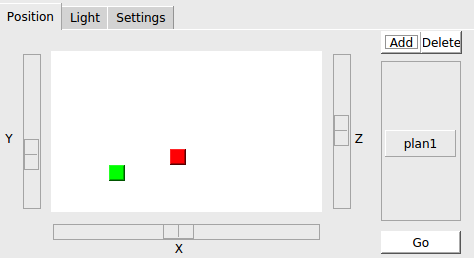
\includegraphics[width=0.9\linewidth]{0_Filer/Figuer/Position.png}
\caption{Position-fane}
\label{fig:GUI Position}
\end{figure}

Position er det første faneblad, der ses når applikationen bliver startet. Alle knapperne der visualiseres på skærmen er angivet i en UI-fil, der hedder "display". I position.cpp vil interaktionen med alle GUI’ens elementer i Position-fanen blive behandlet. Denne fils primære formål er at stå for at sende de beskeder, som motorerne skal modtage for x-, y- og z-aksen videre vha. SPI-kommunikation. Denne styring involverer elementer, som sliders der benyttes af brugeren til at fremstille koordinator, som lampen skal bevæge sig til ved klik på Go-knappen. Klikket på Go-knappen fortæller systemet at beskeden skal sendes videre til PSoC-Master. I denne fane er der ligeledes en rektangulær boks i den højre side. Over denne boks er en Add- og Delete-knap. Ved tryk på Add vil dialogboksen komme frem. Når en plan er oprettet vil denne blive fremvist i den rektangulære boks med et maximum på 4 planer. Hvis en plan er markeret vil et tryk på Delete resultere i at planen bliver nedlagt og ophøre med at eksistere.

\subsubsection{Light}

\begin{figure}[H]
\centering
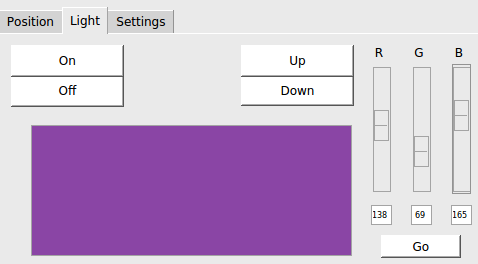
\includegraphics[width=0.9\linewidth]{0_Filer/Figuer/Light.png}
\caption{Light-fane}
\label{fig:GUI Light}
\end{figure}

Light er det andet faneblad fra venstre mod højre, som kan ses i tab-widget menuen. Det er i denne fane, hvor interaktionen med lysstyring foretages. Selve vinduet er bygget op som en del af tab-widgetten i Displays's UI, men det er light.cpp, der står for behandlingen af interaktionerne, der sker i denne fane. 
Nedenfor ses et klassediagram for GUI'en, hvor klasserelationerne kan ses. Det fremgår af klasserelationerne, at Position som primære fil står for at hente data fra GUI'en og brugerens interaktionen med den, hvilket hovedsagligt foregår med signals \& slots. Signals \& slots er GUI'ens interne eventhandler. Når et event sker, sendes dette signal til dette slot (funktion) som udfører det og det. QT er et eventbaseret system, så opbygningen af den er primært bestående af forståelsen for hvordan delelementer snakker sammen, eller snarer hvordan man får dem til at snakke sammen. Arv og pointerlogik spiller her en stor rolle.

\subsubsection{Settings}

\begin{figure}[H]
\centering
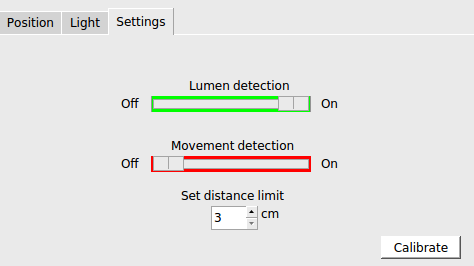
\includegraphics[width=0.9\linewidth]{0_Filer/Figuer/Settings.png}
\caption{Settings-fane}
\label{fig:GUI Settings}
\end{figure}

Settings er det tredje faneblad fra venstre mod højre. Denne fane har til ansvar at sætte sensorindstillingerne. Disse sensorer indbefatter afstandssensor, bevælgelsessensor og lumensensor. Bevægelsessensoren og lumensensoren er helt simplistisk bestående af sliders som kan sættes til minumum, der beskriver tilstanden Off, eller maksimum, der beskriver tilstande On. Når disse er On, betyder det at sensorne er aktive og deres respons påvirker udfaldsforløbet for det samlede system. Afstandssensoren er opbygget af en spinbox, hvori man kan indstille hvilken afstand den skal registrere at et objekt er for tæt på. Dette er en heltalsværdi med et minimum på 3 og et maximum på 255 med enheden centimeter. Det er også i denne fane at kalibreringsknappen ”Calibrate” kan findes. Calibrate er noget brugeren kan benytte til at rette op på uoverensstemmelser i positionering hvis denne er skredet fra det forventet. Dette påbegynder en bevægelsesrutine og lagrer ved afslutning nogle calibreringsdata på de respektive slave PSoC'er, PSoC-XY og PSoC-Z.

\subsubsection{PlannerDialog og planner}

\begin{figure}[H]
\centering
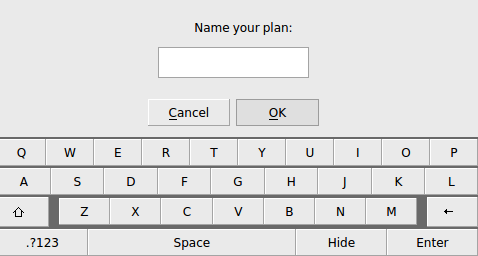
\includegraphics[width=0.9\linewidth]{0_Filer/Figuer/plannerDialog.png}
\caption{Settings-fane}
\label{fig:GUI Dialog}
\end{figure}

Plannerdialogboksen er den dialogboks der bringes frem, når man trykker på Add-knappen, hvis brugeren vælger at oprette en plan. Dialogboksen indeholder et tekstfelt hvori navnet på planen indtastes. Der kan heri indtastes alle tegntyper begrænset til maksimalt 8-tegn. Dette antal er valgt, for at de oprettede knapper har et navn der fylder maksimalt en linje med en skriftstørrelse, der vil være læsbar på en skærm af den størrelse der benyttes til dette produkt (480*272). Alt over 8-tegn ville kræve at skriftstørrelsen skulle være mindre eller der skulle laves linjeskift, hvilket ikke ville være hensigtsmæssigt. Indtastningen i indtastningsfeltet gøres vha. af det virtuelle keyboard, der befinder sig i den nederste halvdel af skærmen i dialogboksen. 

Keyboardet er ikke lavet af denne gruppe, men er blevet downloadet og implementeret fra "the Free Software Foundation". Keyboardet er dog blevet modificeret i størrelse og indtastningsvenlighed, og "Hide"-knappen der oprindeligt benyttes til at skjule keyboardet er blevet gjort funktionsløst, da denne funktionalitet var unødvendig for dette produkt. For mere information om dette keyboard samt et downloadlink til det kan ses fra følgende reference \footcite{qtvirtkey}. Under indtastningsfeltet kan findes en Ok- og Cancel-knap. Tryk på Ok-knappen opretter planen med det indtastede navn, hvorimod Cancel-knappen annulerer oprettelse af plan og returnerer brugeren til den forhenværende brugerflade. For at undgå at navneløse planer bliver oprettet er Ok-knappen disablet indtil mindst et eller flere tegn indtastes i indtastningsfeltet. Der er en begrænsning på mængden af planer på 4, da dette var den maksimale mængde, der var plads til foruden knapstørrelsen skulle formindskes. Hvis en plan ønskes fjernet skal brugeren trykke på givne plan og trykke på Delete-knappen placeret ved siden af Add-knappen.

% 6.1.2.4 Klassebeskrivelser Devkit8000
\subsection{Klassebeskrivelse Devkit8000}

MainDisplay er den første UI der kan ses, som åbnes, når applikationen startes og er den eneste, som forbliver åbent. Det er applikationens primære UI-fil, hvor den hovedsaglige interaktion foretages og fungerer som bindeled for GUI'ens klasser. Denne widget indeholder en stor række af GUI'ens funktionaliteter, da GUI'en blev opbygget i faner i stedet for i separate QWidgets (Applikationsvinduer). MainDisplay's UI-fil indeholder den grundlæggende funktionalitet, som er nødvendig for at oprette vinduet.
\newline

Nedenfor ses et klassediagram for GUI’en, hvor det fremgår, at MainDisplay er den ledende klasse med det UI, som de andre klasser bruges i. Det fremgår af klasserelationen, at MainDisplay som QWidget anvender GUI’ens resterende klasser, hvilket hovedsagligt foregår med signals \& slots. Position, Planner, Light og Settings har ikke deres egne QWidget klasser, da de alle er bygget på MainDisplay QWidgeten, hvilket har resulteret i en stor samling af metoder i en fil.

\begin{figure}[H] \centering
    \fbox{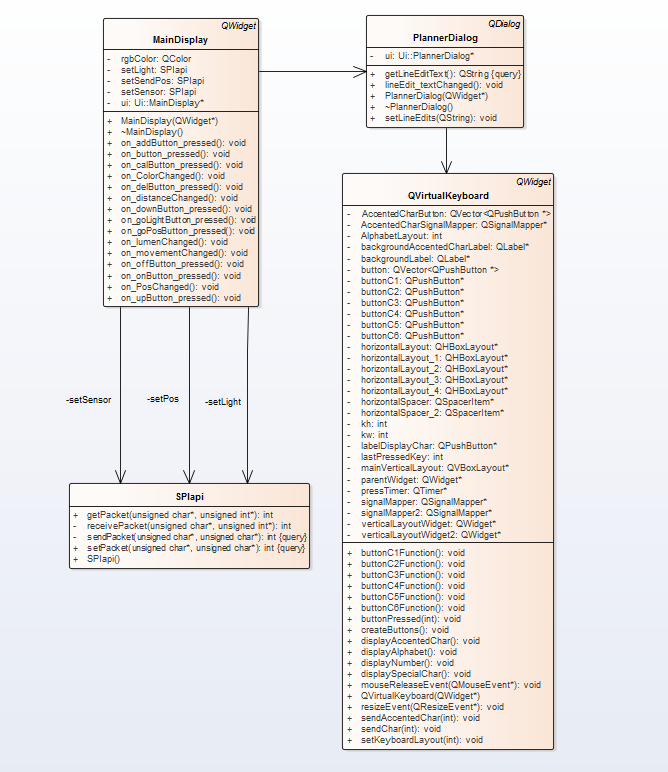
\includegraphics[width=0.95\textwidth]{0_Filer/Figuer/guiClassDia.png}}
    \caption{GUI klassediagram genereret vha. Enterprise Architect}
    \label{fig:GUI klassediagram}
\end{figure}

% 6.1.2.5 GUI repræsentationsbeskrivelse
\subsection{GUI repræsentationsbeskrivelse}

Klassen MainDisplay, der kan forefindes i maindisplay.h, indeholder metoder fra følgende filer:
\begin{itemize}
\item display.ui
\item position.cpp
\item planner.cpp
\item light.cpp
\item settings.cpp
\end{itemize}

Klassen PlannerDialog, der kan forefindes i plannerdialog.h, indeholder metoder fra følgende filer:
\begin{itemize}
\item plannerdialog.ui
\item plannerdialog.cpp
\end{itemize}

GUI-filen repræsenterer et vindue bestående af følgende elementer:
\begin{itemize}

\item Tab Widget - Indeholder tre separate faner: Position, Light og Settings.

\item Sliders (Position-fane) – Til indstilling af lampens position i X-, Y- og Z-aksen i trin mellem 0 og 255.

\item Go-knap (Position-fane) – Til at udsende sliderværdierne for X, Y og Z til bevægelse af lampe.

\item Add-knap (Position-fane) - Til åbne dialogboksen til oprettelse af en plan.

\item Sliders (Light-fane) - Til indstilling af farven der udsendes til lampen i trin mellem 0 og 255.

\item Trinbokse (Light-fane og Position-fane) - Til visning af sliders trinværdi.

\item Farvepalette (Light-fane) - Hvor indstillede farve vises, der forventes at blive vist på lysenhed.

\item On/Off-knapper (Light-fane) – On-knap til at sætte RGB-LED’erne på sidste lysindstilling forinden den blev slukket og Off-knap for at slukke lyset.

\item Up/Down-knapper (Light-fane) - Bruges til at flytte farvesliders enten op eller ned med 5 steps.

\item Labels – Position: X, Y og Z til identifikation af hvilken slider der kontrollerer hvilken akse. Light: R, G og B til identifikation af sliders for farverne rød, grøn og blå.

\item Plot – Et X-, Y-koordinatsystem til visualisering af lampens nuværende position (med grønt ikon) og dens kommende position (rødt ikon), hvis sliders er blevet flyttet.

\item Lumen slider (Settings-fane) - En slider til at sende en tænd- eller slukbesked til lyssensoren.

\item Movement slider (Setttings-fane) - En slider til at sende en tænd- eller slukbesked til bevægelsessensoren.

\item Distance spinbox (Settings-fane) - En spinbox der sætter den værdi hvorindenfor afstandssensoren sender en advarsel.

\item Calibrate-knap (Settings-fane) - Starter kalibreringsprocessen ved tryk.

\end{itemize}

I constructoren til klassen MainDisplay sker opsætningen af GUI'en, når den startes. Her får vi komponenter fra UI'et til at kommunikere sammen med signals \& slots. Dette gøres vha. connect() metoder, så der kan emittes signaler, hvorefter de tilhørende slots kaldes. I dette specifikke kodeudsnit ses hvordan slidernes signaler er blevet sat op. Alle sliderne fra de tre faner connectes samtidig. Position, Light og Settings er dermed klar til intern kommunikation forinden metoderne kaldes.

\begin{figure}[H]
\centering
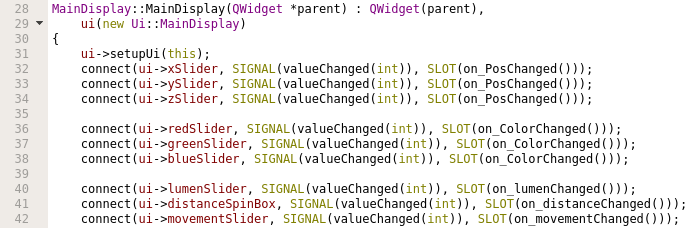
\includegraphics[width=0.9\linewidth]{0_Filer/Figuer/signalSlot.png}
\caption{Kodeudsnit af Signals \& Slots i MainDisplay's constructor}
\label{fig:signalSlot}
\end{figure}

\subsection{GUI modultest}
Der er blevet foretaget en række forskellige test på GUI'en for at sikre at alle funktionerne har de korrekte funktionaliteter. Koden indeholder en række metoder og interne signaler, der skal sendes rigtigt hele vejen igennem systemet for at sikre, at resten af systemet vil kunne bruge disse. GUI test er primært blevet fortaget med QDebugger, som er blevet brugt til at udskrive data og tekststrenge så kodeeksekveringen kunne følges. \newline

\begin{table}[H]
\begin{tabular}{|l|l|}\hline
\textbf{Test} & Positionsindstilling ved sliderændringer \\\hline

\textbf{Testbeskrivelse} & \multicolumn{1}{|m{11.5cm}|}{Der testes, om ændring af X-, Y- og Z-sliders positioner sætter nogle værdier og om de bliver sendt korrekt ved tryk på Go-knap.  QDebug() bruges til at udskrive positionsværdierne i metoden on\_PosChanged(), der kaldes ved valueChanged(int).} \\\hline


\textbf{Input} & \multicolumn{1}{|m{11.5cm}|}{Sliders positioner ændres til hhv. 255, 255, 255. Derefter trykkes Go-knappen ned og slippes igen.} \\\hline

\textbf{Output} & \multicolumn{1}{|m{11.5cm}|}{ Sliderpositionen og nuværende position vil ændre sig til "255, 255, 255", blive udskrevet og de negative kommandokoder vil blive returneret som fejlkoder (X=16, Y=17, Z=32).} \\\hline

\textbf{Resultat} & \multicolumn{1}{|m{11.5cm}|}{ OK} \\\hline

\end{tabular}
\end{table}

\begin{figure}[H]
\centering
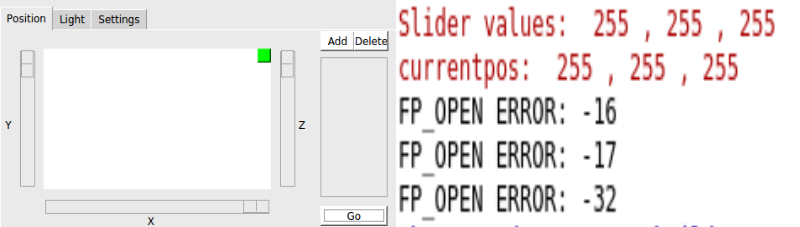
\includegraphics[width=1.0\linewidth]{0_Filer/Figuer/testPosition.png}
\caption{Debug output ved sliderværdierne (X, Y, Z): 255, 255, 255, den sendte værdi currentpos: 255, 255, 255 og negative sendte kommandoer.}
\label{fig:testPosition}
\end{figure}


\begin{table}[H]
\begin{tabular}{|l|l|}\hline
\textbf{Test} & Lysindstilling ved sliderændringer \\\hline

\textbf{Testbeskrivelse} & \multicolumn{1}{|m{11.5cm}|}{Det testes, om ændring af R-, G- og B-sliders positioner sætter nogle værdier og om de bliver sendt korrekt ved tryk på Go-knap.  QDebug() bruges til at udskrive positionsværdierne i metoden on\_ColorChanged(), der kaldes ved valueChanged(int).} \\\hline

\textbf{Input} & \multicolumn{1}{|m{11.5cm}|}{Sliders positioner ændres til hhv. 255, 255, 255. Derefter trykkes Go-knappen ned og slippes igen.} \\\hline

\textbf{Output} & \multicolumn{1}{|m{11.5cm}|}{ Sliderpositionen og sendte lysværdi vil ændre sig til "255, 255, 255", blive udskrevet og de negative kommandokoder vil blive returneret som fejlkoder (R=48, G=49, B=50).} \\\hline

\textbf{Resultat} & \multicolumn{1}{|m{11.5cm}|}{ OK} \\\hline

\end{tabular}
\end{table}

\begin{figure}[H]
\centering
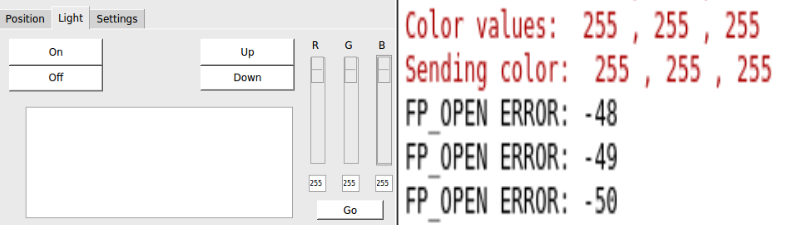
\includegraphics[width=1.0\linewidth]{0_Filer/Figuer/testLight.png}
\caption{Debug output ved sliderværdierne Color values (R, G, B): 255, 255, 255, den sendte værdi Sending color: 255, 255, 255 og negative sendte kommandoer.}
\label{fig:testLight}
\end{figure}



\begin{table}[H]
\begin{tabular}{|l|l|}\hline
\textbf{Test} & Sensorindstilling ved slider og spinboxændringer \\\hline

\textbf{Testbeskrivelse} & \multicolumn{1}{|m{11.5cm}|}{Det testes, om ændring af Movementslider, Lumensensor samt Distancespinbox bliver sendt videre med SPI kommandoer.} \\\hline

\textbf{Input} & \multicolumn{1}{|m{11.5cm}|}{Sliders position for Movement og Lumen ændres fra Off til On. Derefter ændres Distancespinboxværdien til 4.} \\\hline

\textbf{Output} & \multicolumn{1}{|m{11.5cm}|}{ Sliderpositioner for Lumen og Movement ændres til On, status bliver udskrevet og de negative kommandokoder vil blive returneret som fejlkoder (R=48, G=49, B=50).} \\\hline

\textbf{Resultat} & \multicolumn{1}{|m{11.5cm}|}{ OK} \\\hline

\end{tabular}
\end{table}

\begin{figure}[H]
\centering
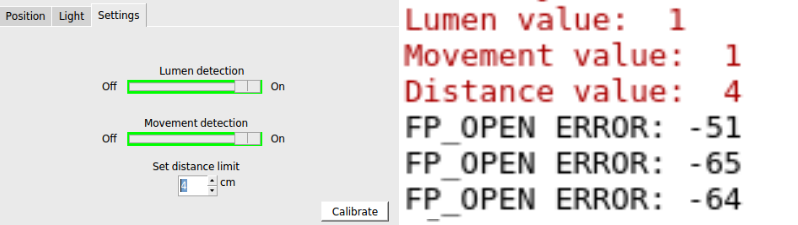
\includegraphics[width=1.0\linewidth]{0_Filer/Figuer/testSettings.png}
\caption{Debug output ved sliderværdierne Lumen value: 1, Movement value: 1, spinboxværdien Distance value: 4 og negative sendte kommandoer.}
\label{fig:testSettings}
\end{figure}



\begin{table}[H]
\begin{tabular}{|l|l|}\hline
\textbf{Test} & Oprettelse af plan \\\hline

\textbf{Testbeskrivelse} & \multicolumn{1}{|m{11.5cm}|}{Det testes, om der kan oprettes en plan og de korrekte værdier gemmes.} \\\hline

\textbf{Input} & \multicolumn{1}{|m{11.5cm}|}{Sliderposition for X, Y og Z ændres til "255, 255, 255" og R, G, og B ændres til "255, 0, 0". Der trykkes dernæst op Add-knappen, et navn indtastes i dialogboksen der fremvises på skærmen og Ok-knappen trykkes.} \\\hline

\textbf{Output} & \multicolumn{1}{|m{11.5cm}|}{Plannens positionsvædier sættes til "255, 255, 255" og lysværdierne sættes til "255, 0, 0". Disse værdier udskrives i debuggeren.} \\\hline

\textbf{Resultat} & \multicolumn{1}{|m{11.5cm}|}{ OK} \\\hline

\end{tabular}
\end{table}

\begin{figure}[H]
\centering
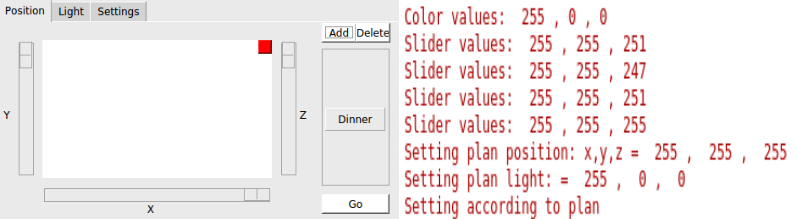
\includegraphics[width=1.0\linewidth]{0_Filer/Figuer/testMakePlan.png}
\caption{Debug output ved satte plan X, Y og Z Setting plan position: (255, 255, 255), lyset R, G, B Setting plan Light (255, 0, 0) og Setting according to plan}
\label{fig:testmakePlan}
\end{figure}
